\pdfoutput=1
\pdfminorversion=6
\documentclass{article}

% if you need to pass options to natbib, use, e.g.:
%\PassOptionsToPackage{numbers, compress}{natbib}
% before loading neurips_2024

\PassOptionsToPackage{numbers, compress}{natbib}
\bibliographystyle{plainnat}

% ready for submission
%\usepackage[preprint]{neurips_2024}


% to compile a preprint version, e.g., for submission to arXiv, add add the
% [preprint] option:
%     \usepackage[preprint]{neurips_2024}


% to compile a camera-ready version, add the [final] option, e.g.:
%     \usepackage[final]{neurips_2024}


% to avoid loading the natbib package, add option nonatbib:
\usepackage[preprint]{neurips_2023}

\usepackage[utf8]{inputenc} % allow utf-8 input
\usepackage[T1]{fontenc}    % use 8-bit T1 fonts
\usepackage{adjustbox}

\usepackage{booktabs}       % professional-quality tables
\usepackage{amsfonts}       % blackboard math symbols
\usepackage{nicefrac}       % compact symbols for 1/2, etc.
\usepackage{microtype} 
\usepackage{graphicx}
\usepackage{hyperref}  

\usepackage{caption}
\usepackage{grffile}
\usepackage{url}            % simple URL typesetting
\usepackage{subcaption}
\usepackage{wrapfig}
\usepackage[dvipsnames]{xcolor}      % colors
\usepackage{multirow}
\usepackage{dsfont}
\usepackage[most]{tcolorbox}
\usepackage{enumitem}
\usepackage{listings}
\hypersetup{
    colorlinks = true,
    citecolor = BlueViolet,
    linkcolor = BrickRed
}
\usepackage{pythonhighlight}

\newcommand\blfootnote[1]{%
  \begingroup
  \renewcommand\thefootnote{}\footnote{#1}%
  \addtocounter{footnote}{-1}%
  \endgroup
}

% \title{Automatic jailbreaking the Image Generative AI}
\title{Automatic Jailbreaking of the\\ Text-to-Image Generative AI Systems}


% The \author macro works with any number of authors. There are two commands
% used to separate the names and addresses of multiple authors: \And and \AND.
%
% Using \And between authors leaves it to LaTeX to determine where to break the
% lines. Using \AND forces a line break at that point. So, if LaTeX puts 3 of 4
% authors names on the first line, and the last on the second line, try using
% \AND instead of \And before the third author name.


\author{%
    Minseon Kim$^1$, Hyomin Lee$^2$, Boqing Gong$^3$, Huishuai Zhang$^4$, Sung Ju Hwang$^{1,5}$ \\
    $^1$KAIST, $^2$Korea University, $^4$Peiking University $^5$DeepAuto.ai \\
    \texttt{\{minseonkim, sjhwang82\}@kaist.ac.kr,} 
    \texttt{lhm1024@korea.ac.kr,} \\
    \texttt{boqinggo@outlook.com, zhanghuishuai@pku.edu.cn}
}


\begin{document}

%\usepackage{natbib}
\maketitle

\begin{abstract}
Diffusion Models have emerged as powerful generative models for high-quality image synthesis, with many subsequent image editing techniques based on them. However, the ease of text-based image editing introduces significant risks, such as malicious editing for scams or intellectual property infringement. Previous works have attempted to safeguard images from diffusion-based editing by adding imperceptible perturbations. These methods are costly and specifically target prevalent Latent Diffusion Models (LDMs), while Pixel-domain Diffusion Models (PDMs) remain largely unexplored and robust against such attacks. Our work addresses this gap by proposing a novel attacking framework with a feature representation attack loss that exploits vulnerabilities in denoising UNets and a latent optimization strategy to enhance the naturalness of protected images. Extensive experiments demonstrate the effectiveness of our approach in attacking dominant PDM-based editing methods (e.g., SDEdit) while maintaining reasonable protection fidelity and robustness against common defense methods. Additionally, our framework is extensible to LDMs, achieving comparable performance to existing approaches.
\end{abstract}

\section{Introduction}
%
Large Transformers have enabled a number of breakthrough advances in modeling language, vision, audio, biology and numerous other domains \citep{vaswani2017attention}, \citep{dosovitskiy2020image}, \citep{radford2022robust}, \citep{cramer2021alphafold2}. Much of the success of Transformers, powered by the attention operator \citep{vaswani2017attention}, relies on their scaling properties \citep{hoffmann2022training} and the emergence of in-context learning \citep{garg2022can}, which allows them to generalize to unseen data and tasks given context as input. 
%
The Transformer block is a powerful tool for sequence modeling, but it is not without its limitations. One of the most notable is the computational cost, which grows rapidly as the length of the input sequence increases. Specifically, the cost scales quadratically with the length $L$ of the sequence, which places a strict limit on the amount of context that can be considered by the model.
%
Breaking the quadratic barrier is a key step towards new possibilities for deep learning, such as using entire textbooks as context, generating long-form music or processing gigapixel scale images.

Efforts to reduce the computational cost of attention in models primarily involve the use of linearized, low-rank, and sparse approximations \citep{child2019generating,wang2020linformer,kitaev2020reformer,zhai2021attention,roy2021efficient,schlag2021linear,tu2022maxvit}. These approaches introduce a trade-off between expressivity and speed, requiring hybridization with standard attention layers to reach Transformer quality \citep{mehta2022long,dao2022hungry}.

A growing amount of evidence suggests that attention mechanisms only utilize a small portion of their quadratic capabilities for language processing \citep{olsson2022context, dao2022hungry}, leading us to question its role as the gold-standard operator for deep learning at scale. Specifically, we ask:

%
\begin{figure*}[t]
    \centering
    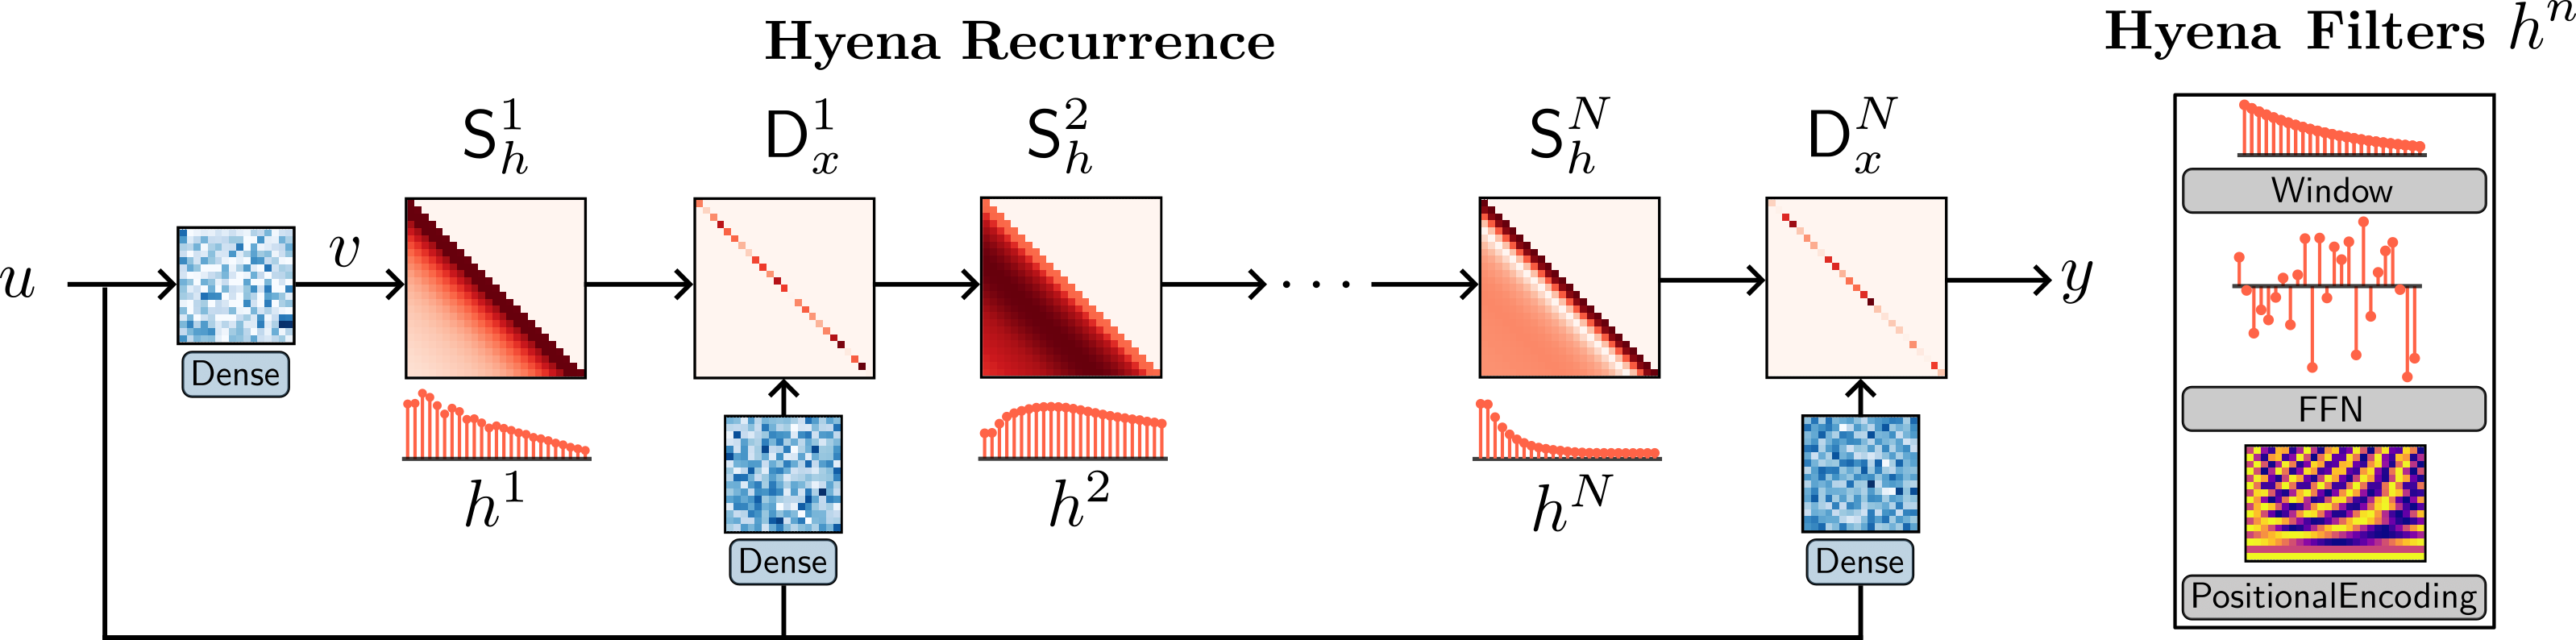
\includegraphics[width=\linewidth]{figures/hyena.png}
    \vspace{-2mm}
    \caption{The ${\sf Hyena}$ operator is defined as a recurrence of two efficient subquadratic primitives: an implicit long convolution $h$ (i.e. {\sf Hyena} filters parameterized by a feed-forward network) and multiplicative element-wise gating of the (projected) input. The depth of the recurrence specifies the size of the operator. {\sf Hyena} can equivalently be expressed as a multiplication with \textit{data-controlled} (conditioned by the input $u$) diagonal matrices $\sD_x$ and Toeplitz matrices $\sS_h$. In addition, {\sf Hyena} exhibits sublinear parameter scaling (in sequence length) and unrestricted context, similar to attention, while having lower time complexity.}
    \label{arch}
\end{figure*}
%

{\centering
\textit{Are there subquadratic operators that can match the quality of attention at scale?}\par}

\vspace{0.5cm}
% 

We obtain a positive answer based on a composition of efficient subquadratic primitives, such as \textit{element-wise multiplication} (gating) and \textit{long convolutions} i.e., convolutions with filter sizes as long as the input. We rely on a set of targeted reasoning tasks, grounded in recent work on \textit{mechanistic interpretability} \citep{elhage2021mathematical,power2022grokking,olsson2022context,zhang2022unveiling} such as recall and induction, to distill three properties of attention correlated with its performance and the quality gap with existing subquadratic approaches: 
%
\begin{itemize}[leftmargin=0.1in]
    \item[$a.$] \textbf{Data control:} Attention implements an expressive \textit{data-controlled} \citep{massaroli2020dissecting} linear operator\footnote{Self-attention can be expressed as $y = \sA(k, q) v$ where $\sA$ is the \textit{attention matrix} conditioned by linear projections $k, q$ of the input and multiplied by $v$, another projection.}, encoding an entire family of linear functions in a single block.
    \item[$b.$] \textbf{Sublinear parameter scaling:} Parameter counts of attention layers are decoupled from sequence length, allowing Transformers to allocate more parameters elsewhere e.g., the \textit{feed-forward neural networks} ({$\sf FFN$s}) between attention layers.
    \item[$c.$] \textbf{Unrestricted context:} For a given input, attention has an unrestricted context i.e., it can approximate dependencies between any two inputs, without arbitrary restrictions such as locality (except in cases using masking such as autoregressive models).
\end{itemize}
%
\paragraph{The ${\sf Hyena}$ hierarchy}
%
Guided by these findings, we introduce the ${\sf Hyena}$ hierarchy, an operator defined by a recurrence of two efficient subquadratic primitives: \textbf{a long convolution and element-wise multiplicative gating} (see Figure \ref{arch}). A specified depth (i.e., number of steps) of the recurrence controls the size of the operator. For short recurrences, existing models are recovered as special cases \citep{mehta2022long,dao2022hungry}. By mapping each step in the ${\sf Hyena}$ recurrence to its corresponding matrix form, we reveal ${\sf Hyena}$ operators to be equivalently defined as a decomposition of a \textit{data-controlled} matrix i.e., a matrix whose entries are functions of the input. Furthermore, we show how ${\sf Hyena}$ operators can be evaluated efficiently without materializing the full matrix, by leveraging fast convolution algorithms \citep{selesnick2017fast}. Empirically, ${\sf Hyena}$ operators are able to significantly shrink the quality gap with attention at scale, reaching similar perplexity and downstream performance with a smaller computational budget (Section \ref{res:lm}) and \textbf{without hybridization} of attention.
%

\paragraph{Narrowing the capabilities gap}
%
The design of {\sf Hyena} is motivated by a quality gap between standard dense attention and alternative subquadratic operators, which we identify by focusing on reasoning tasks correlated with language modeling performance at scale. We extend the suite of basic mechanistic interpretability benchmarks (\textit{induction} and \textit{recall}) with additional tasks that probe how quickly model performance degrades when task complexity increases (e.g. vocabulary size grows). In addition, we investigate the optimal parameterization of long convolutions in ${\sf Hyena}$. In the most challenging settings with hundreds of thousands of tokens, our implicit parameterization scheme improves over other operators leveraging state spaces \citep{gu2021efficiently}, frequency-domain parametrizations \citep{li2020fourier}, or standard convolutions by over $50\%$ accuracy.
%
\paragraph{Scaling in language and vision}
%
Next, we aim to verify whether rankings in our reasoning benchmark suite are predictive of quality at scale. We test ${\sf Hyena}$ on autoregressive language modeling at the sub-billion parameter scale, setting a new state-of-the-art for dense-attention-free architectures in standard datasets ({\sc WikiText103} and {\sc The Pile}) and matching Transformer quality. On the {\sc The Pile} at the $335$M parameter scale, we match Transformer perplexity with a $20\%$ reduction in the total count of \textit{floating point operations} (FLOPs). As an extension, we investigate the generality of ${\sf Hyena}$ operators by testing on large-scale image recognition, replacing attention in the Vision Transformer (ViT) \citep{dosovitskiy2020image}. In image classification, ${\sf Hyena}$ is able to match attention in accuracy when training on ImageNet-1k from scratch.
%
\paragraph{Toward much longer context}
%
Finally, we benchmark the efficiency of ${\sf Hyena}$ on long sequences. We measure $5$x speedups over dense self-attention at length $8192$ -- $2$x over highly optimized FlashAttention\footnote{FlashAttention is already 2-4x faster than a standard attention implementation in PyTorch.} \citep{dao2022flashattention} -- and $100$x speedup over FlashAttention at sequence lengths of $64$k, where standard attention implementation in PyTorch runs out of memory. 
\vspace{-0.1in}
\section{Preliminary}
\vspace{-0.1in}
%The issue of copyright infringement in text-to-image (T2I) models has gained significant attention as these models become more prevalent. Early studies, such as those by Heikkilä [1], highlighted the risks of T2I models replicating copyrighted images from detailed prompts, emphasizing the need for robust prevention mechanisms. O'Leary [2] discussed the ethical and legal challenges of AI-generated content, advocating for clearer guidelines and regulations. Vincent [3] demonstrated that even general prompts could lead T2I models to generate images similar to copyrighted content, suggesting solutions like filtering training data and post-generation checks. Gao et al. [4] developed an adversarial attack framework to test T2I models, revealing vulnerabilities in many commercial services and calling for improved robustness and compliance protocols.
\paragraph{Copyright.}
Copyright is a legal protection provided to the owners of "original works of authorship", such as literature, music, and art~\citep{uscopyright2024uscopyright, uspto2024copyright}. This protection is granted to owners under the laws with the \textit{exclusive right to reproduce, or distribute} their works for a certain period of time~\citep{cornell106, uscopyright2024uscopyright}. Reproduction includes making copies of the work in any form, and distribution involves making the work available to the public through selling or lending copies. While the use of copyrighted data in AI models has been tacitly accepted for educational purposes, the rise of commercial AI systems has brought significant attention to the issue of copyright infringement~\citep{lawsuit1,lawsuit2NYTimes,lawsuit3Getty}. Opinions on the legal aspects of AI vary, but ethically, generative AI should not violate any of these rights to protect the intellectual property of the owners. 
In academia, numerous efforts have been made for copyright protection, e.g., training data protection~\citep{zhong2023copyright, shan2023glaze}, theoretical guarantees~\citep{bousquet2020synthetic, elkin2023can, vyas2023provable}, guided generation~\citep{schramowski2022safe, kumari2023ablating} and mechanism design~\citep{zhou2024plug, golatkar2024cpr, deng2024economic}. Despite the efforts, we reveals that commercial T2I systems still infringe copyrights despite careful alignment and red-teaming mechanisms. %Our result also suggests that future protection approaches should be studied under the context of carefully constructed prompts from strong attackers. 

\vspace{-0.12in}
\paragraph{Memorization in T2I models.}
Memorization has been known to occur in T2I models, sometimes producing near-exact reproductions of images from the training dataset~\citep{somepalli2023understanding}.~\citet{carlini2023extractdm} introduce the membership inference attack to extract the training dataset of diffusion models, and several works~\citep{somepalli2023diffusion, wen2024detecting, wang2024diagnosis} have been proposed to mitigate these memorization issues. Despite memorization is a well-known phenomenon, the quantitative evaluation of copyright violation in commercial T2I systems is under-explored. Thus, we propose an Automatic Prompt Generation Pipeline (APGP) to induce copyright infringement in these commercial T2I systems to evaluate the copyright violation using a single target image.

\vspace{-0.12in}
\paragraph{Prompt attack in T2I models.}
Previous attack approaches demonstrate the vulnerabilities in T2I diffusion models by attacking prompts to either generate different objects~\citep{maus2023black} or create potentially harmful images~\citep{yang2023sneakyprompt, zhai2024discovering}. Previous studies~\citep{zhang2023investigating} have explored high-risk prompts that increase copyright risks by pruning tokens based on attention scores, highlighting potential copyright risks but not causing direct infringement. In contrast, our method targets commercial T2I systems without accessing their weights, effectively "jailbreaking" these systems to demonstrate vulnerabilities related to exact copyright infringement.
\section{Method}
\label{sec:method}

\subsection{Practical choice of diffusion paradigm}
\label{subsec:practical_dwm}

Building on the background provided in Section \ref{sec:framework}, we now introduce \textsc{diamond} as a practical realization of a diffusion-based world model. In particular, we now define the drift and diffusion coefficients $\mathbf{f}$ and $g$ introduced in Section \ref{subsec:diffusion}, corresponding to a particular choice of diffusion paradigm. While \textsc{ddpm} \citep{ho2020DDPM} is an example of one such choice (as described in Appendix \ref{app:ddpm}) and would historically be the natural candidate, we instead build upon the \textsc{edm} formulation proposed in \citet{karras2022elucidating}. The practical implications of this choice are discussed in Section \ref{subsec:diffusion_choice}. In what follows, we describe how we adapt \textsc{edm} to build our diffusion-based world model.

We consider the perturbation kernel $p^{0\tau}(\x_{t+1}^\tau \mid \x_{t+1}^0) = \mathcal{N}(\x_{t+1}^\tau; \x_{t+1}^0, \sigma^2(\tau) \mathbf{I})$, where $\sigma(\tau)$ is a real-valued function of diffusion time called the noise schedule. This corresponds to setting the drift and diffusion coefficients to $\mathbf{f}(\x, \tau) = \mathbf{0}$ (affine) and $g(\tau) = \sqrt{2 \dot \sigma(\tau) \sigma(\tau)}$.

We use the network preconditioning introduced by \citet{karras2022elucidating} and so parameterize $\mathbf{D}_\theta$ in Equation \ref{eq:denoising_sm_conditional} as the weighted sum of the noised observation and the prediction of a neural network $\mathbf{F}_\theta$,
\begin{equation}
\label{eq:karras_wrappers} 
    \mathbf{D}_\theta(\x_{t+1}^\tau, y_t^\tau) = c_\text{skip}^\tau \; \x_{t+1}^\tau + c_\text{out}^\tau \; \mathbf{F}_\theta \big( c_\text{in}^\tau \; \x_{t+1}^\tau, y_t^\tau \big),
\end{equation}
where for brevity we define $y_t^\tau \coloneqq (c_\text{noise}^\tau, \x^0_{\le t}, a_{\le t})$ to include all conditioning variables.

The preconditioners $c_\text{in}^\tau$ and $c_\text{out}^\tau$ are selected to keep the network's input and output at unit variance for any noise level $\sigma(\tau)$, $c_\text{noise}^\tau$ is an empirical transformation of the noise level, and $c_\text{skip}^\tau$ is given in terms of $\sigma(\tau)$ and the standard deviation of the data distribution $\sigma_\text{data}$, as $c_{skip}^\tau = \sigma_{data}^2/(\sigma_{data}^2 + \sigma^2(\tau))$. These preconditioners are fully described in Appendix \ref{appendix:karras_conditioners}.

Combining Equations \ref{eq:denoising_sm_conditional} and \ref{eq:karras_wrappers} provides insight into the training objective of $\mathbf{F}_\theta$,
\begin{align}
\label{eq:effective_obj}
\mathcal{L}(\theta)  = \bbe \Big[ \Vert 
\underbrace{\mathbf{F}_\theta \big( c_\text{in}^\tau \x_{t+1}^\tau, y_t^\tau \big)}_\text{Network prediction} - 
\underbrace{\frac{1}{c_\text{out}^\tau} \big( \x_{t+1}^0 - c_\text{skip}^\tau \x_{t+1}^\tau\big)}_\text{Network training target}
\Vert^2 \Big].
\end{align}
The network training target adaptively mixes signal and noise depending on the degradation level $\sigma(\tau)$.
When $\sigma(\tau) \gg \sigma_\text{data}$, we have $c_\text{skip}^\tau \to 0$, and the training target for $\mathbf{F}_\theta$ is dominated by the clean signal $\x_{t+1}^0$. Conversely, when the noise level is low, $\sigma(\tau) \to 0$, we have $c_\text{skip}^\tau \to 1$, and the target becomes the difference between the clean and the perturbed signal, i.e. the added Gaussian noise. Intuitively, this prevents the training objective to become trivial in the low-noise regime. In practice, this objective is high variance at the extremes of the noise schedule, so \citet{karras2022elucidating} sample the noise level $\sigma(\tau)$ from an empirically chosen log-normal distribution in order to concentrate the training around medium-noise regions, as described in Appendix \ref{appendix:karras_conditioners}.

We use a standard U-Net 2D for the vector field $\mathbf{F}_\theta$ \citep{ronneberger2015unet}, and we keep a buffer of $L$ past observations and actions that we use to condition the model. We concatenate these past observations to the next noisy observation channel-wise, and we input actions through adaptive group normalization layers \citep{adagn} in the residual blocks \citep{He2015} of the U-Net.

As discussed in Section \ref{subsec:dwm_training} and Appendix \ref{appendix:sampling}, there are many possible sampling methods to generate the next observation from the trained diffusion model. While our codebase supports a variety of sampling schemes, we found Euler's method to be effective without incurring the cost of additional NFE required by higher order samplers, or the unnecessary complexity of stochastic sampling.

\subsection{Reinforcement learning in imagination}
\label{subsec:rl}

Given the diffusion model from Section \ref{subsec:practical_dwm}, we now complete our world model with a reward and termination model, required for training an RL agent in imagination. Since estimating the reward and termination are scalar prediction problems, we use a separate model $R_\psi$ consisting of standard \textsc{cnn} \citep{cnn_lecun,He2015} and \textsc{lstm} \citep{lstm,Gers2000} layers to handle partial observability. The RL agent involves an actor-critic network parameterized by a shared \textsc{cnn-lstm} with policy and value heads. The policy $\pi_\phi$ is trained with \textsc{reinforce} with a value baseline, and we use a Bellman error with $\lambda$-returns to train the value network $V_\phi$, similar to \citet{iris2023}. We train the agent entirely in imagination as described in Section \ref{subsec:pomdp_and_wm}. The agent only interacts with the real environment for data collection. After each collection stage, the current world model is updated by training on all data collected so far. Then, the agent is trained with RL in the updated world model environment, and these steps are repeated. This procedure is detailed in Algorithm \ref{alg:diamond}, and is similar to \citet{kaiser2019atari100k,hafner2020dream,iris2023}. We provide architecture details, hyperparameters, and RL objectives in Appendices \ref{app:architectures}, \ref{app:hyperparams}, \ref{appendix:rl_actor_critic}, respectively.

\section{Results}


\begin{table*}[t]
\setlength{\tabcolsep}{2pt}
% \scriptsize
\footnotesize
    \centering
    \caption{Comparison of our \textit{OpenMath2-Llama} models with other open-weight and open-source models without tool usage. 
    Open-weight base models finetuned with publicly released data are considered as open-source for the purposes of this table.
    }
    \label{tab:main_results}
    \begin{tabular}{lclccccc} 
    \toprule
    \textbf{Category} & \textbf{Params} & \textbf{Model}   &  \textbf{GSM8K} & \textbf{MATH} 
    & \textbf{AMC 2023} & \textbf{AIME 2024} & \textbf{Omni-MATH\footnotemark} \\\midrule

     \multirow{3}*{\begin{tabular}{c} Open\\Weight\\\\\end{tabular}}  & \multirow{6}{*}{$< 10$B }  
          & Qwen2.5-Math-7B-Instruct~\citep{yang2024qwen25mathtechnicalreportmathematical} & 95.2 &  83.6 & 25/40 & \phantom{1}5/30 & 32.3\\ 
          & & Mathstral-7B~\citep{mathstral} & 77.1 & 56.6 & - &  - & - \\ 

          & & Llama3.1-8B-Instruct~\citep{dubey2024llama3herdmodels} & 84.2 & 51.8 & \phantom{1}9/40 & \phantom{1}2/30 & 12.7 \\[0.1ex]  

    \cdashline{1-1}     \cdashline{3-8} \noalign{\vskip 0.7ex}    
    \multirow{3}*{\begin{tabular}{c} Open\\Source\\\\\end{tabular}}
        & & NuminaMath-7B-CoT~\citep{li2024numinamath} & 75.4 & 55.2 &  11/40 & \phantom{0}0/30 & - \\ 
        & & OpenMath2-Llama3.1-8B (ours) & 91.7 & 67.8 & 16/40 & \phantom{0}3/30 & 22.0\\
        & &  \hspace{1in}\textcolor{blue}{+ maj@256}                    & 94.1 & 76.1 & 23/40 & \phantom{0}3/30 & 24.6\\
        \midrule 
    
    \multirow{3}*{\begin{tabular}{c} Open\\Weight\\\\\end{tabular}} & \multirow{6}*{\begin{tabular}{c} \\10\\to\\100B\\\\\end{tabular}}
    & DS-Coder-V2-Lite-Instruct~\citep{deepseekai2024deepseekcoderv2breakingbarrierclosedsource}  & 86.4 & 61.8 & - & \phantom{0}0/30 & 19.7  \\   
    &  & Qwen2.5-Math-72B-Instruct~\citep{yang2024qwen25mathtechnicalreportmathematical} & 95.9& 85.0 & 28/40 & \phantom{0}9/30 & 36.3 \\ 
    & & Llama3.1-70B-Instruct~\citep{dubey2024llama3herdmodels} &  95.8 & 67.9 & 19/40 & \phantom{0}6/30 & 19.0 \\

    \cdashline{1-1}     \cdashline{3-8} \noalign{\vskip 0.7ex}    
    \multirow{2}*{\begin{tabular}{c} Open\\Source\\\\\end{tabular}} 
            & & NuminaMath-72B-CoT~\citep{li2024numinamath} & 91.4  & 68.0 & 21/40 & \phantom{0}1/30 & 28.4 \\ 
        & & OpenMath2-Llama3.1-70B (ours)               & 94.9 & 71.9 & 20/40 & \phantom{0}4/30 & 23.1 \\
        & &  \hspace{1in}\textcolor{blue}{+ maj@256}    & 96.0 & 79.6 & 24/40 & \phantom{0}6/30 & 27.6 \\
    \bottomrule
        
    \end{tabular}
    \vspace{-0.1in}
\end{table*}









\paragraph{Training Details.}
All the models are trained with a batch size of 512, using the AdamW optimizer~\citep{Loshchilov2019DecoupledWD} with a constant learning rate of 2e-5 and a weight decay of 1e-2. 
For the 8B model, we train the model on 1M, 2M, and 5M fair downsampled versions of \dataset to understand the impact of the data scaling.  
Due to computational constraints, we train the 70B model only on the 5M subset with a learning rate of 1e-5. 
The models are trained for 2 epochs, and we save 6 equally spaced checkpoints during the training runs, which are averaged to create the final model (See Appendix~\ref{sec:app_ckpt_avging} for performance gains with checkpoint averaging). 


\paragraph{Evaluation Details.} 
We evaluate our models on a set of common benchmarks that consists of GSM8K (1.3K examples), MATH (5K examples), AMC 2023 (40 examples), AIME 2024 (30 examples), and Omni-MATH (4.4K examples) \citep{omni_math}. These datasets cover a broad spectrum of difficulty levels, ranging from grade school mathematics to advanced competition problems. Unless noted otherwise, all fine-tuned models are assessed in a zero-shot setting with both greedy decoding and majority voting out of 256 sampled solutions with temperature of 0.7 \citep{wang2022self}.

We use GPT-4o \citep{openai2023gpt4} as a judge to compare the ground truth answers with those predicted by our models (the detailed prompt is provided in Appendix \ref{sec:llm-evaluation-judge}). 


\footnotetext{Omni-MATH dataset was released after we finished training our models, so we didn't use it during decontamination. After checking for contamination, we found that about 1.4\% of the test set questions are part of our training data.}





\paragraph{Impact of Data Scaling.} 
Figure~\ref{fig:sft_scale} plots the performance on the MATH test set with the increase in SFT data size. With even the 1M fair-downsampled version of OpenMathInstruct-2, the final model easily outperforms \texttt{Llama3.1-8B-Instruct} and \texttt{NuminaMath-7B-CoT}.  
We observe a consistent gain with an increase in data size, and even at 14M dataset size, we see no signs of saturation in performance gains.

\paragraph{Final Results.} Table~\ref{tab:main_results} presents the results for top-performing, open-weight and open-source models (without tool use). 
The \texttt{OpenMath2-Llama3.1-8B} model, which is finetuned on the full OpenMathInstruct-2 dataset, outperforms or matches \texttt{Llama3.1-8B-Instruct} on all the math reasoning benchmarks.  
Among the open-source models, we outperform the recently released \texttt{NuminaMath-7B-CoT} on all benchmarks as well. 
Finally, among all the presented models, the \texttt{OpenMath2-Llama3.1-8B} is second only to the \texttt{Qwen2.5-Math-7B-Instruct}, which has been trained on more than a trillion synthetically generated math reasoning tokens, and starts with a base model, \texttt{Qwen2.5-Math}, which is about 35\% better than \texttt{Llama3.1-8B-Base}.
\footnote{We are unsure of the $n$-gram based data contamination protocol followed by \texttt{Qwen2.5-Math} given its obvious weakness in detecting paraphrases.}



The \texttt{OpenMath2-Llama3.1-70B} is our strongest performing model which is the \texttt{Llama3.1-70B-Base} model finetuned on the 5M fair downsampled subset of OpenMathInstruct-2. While our 8B model demonstrates strong accuracy gains compared to other LLMs of similar size, the 70B model only shows improvements on a subset of benchmarks. We hypothesize that our data blend or solution format might be more suited for weaker models, since we made all of the design decisions based on the 8B model accuracy on validation subsets.


\vspace{-5pt}
\section{Conclusion}\label{sec:conclusion}
\vspace{-5pt}
We accelerate high-resolution diffusion models by designing deep compression autoencoders to reduce the number of tokens. We proposed two techniques: \textit{residual autoencoding} and \textit{decoupled high-resolution adaptation} to address the challenges brought by the high compression ratio. The resulting new autoencoder family \modelshort demonstrated satisfactory reconstruction accuracy with a spatial compression ratio of up to 128. \modelshort also demonstrated significant training and inference efficiency improvements when applied to latent diffusion models. 

\section*{Acknowledgements}
We thank NVIDIA for donating the DGX machines. We thank MIT-IBM Watson AI Lab, MIT and Amazon Science Hub, MIT AI Hardware Program, and National Science Foundation for supporting this research. 


\bibliography{reference}


\section{Miscellaneous}




\subsection{Generating Solution in OpenMath CoT Format}
\label{sec:app_soln_format}

\begin{figure*}[t]
    \centering
    \begin{tcolorbox}[
    colback=pastelblue!40,
    colframe=pastelblue!50,
    coltitle=pastelpink!50!black,
    colbacktitle=pastelpink!50,
    listing options={language=},
    fonttitle=\bfseries,
    fontupper=\ttfamily,
    halign title=center,         %
    title=Instruct Prompt Template,              %
    boxrule=0.5mm, 
    width=13cm,
]
\footnotesize
\begin{verbatim}
<|begin_of_text|><|start_header_id|>user<|end_header_id|>

FEW-SHOT PROMPTS

Question:
{question}<|eot_id|><|start_header_id|>assistant<|end_header_id|>

{generation}
\end{verbatim}
\end{tcolorbox}
    \caption{Typical \emph{instruct} prompt template used with \texttt{Llama-Instruct} models.}
    \label{fig:instruct_prompt}
\end{figure*}


\begin{figure*}[t]
    \centering
    \begin{tcolorbox}[
    colback=pastelblue!40,
    colframe=pastelblue!50,
    coltitle=pastelpink!50!black,
    colbacktitle=pastelpink!50,
    listing options={language=},
    fonttitle=\bfseries,
    fontupper=\ttfamily,
    halign title=center,         %
    title=Base Prompt Template,              %
    boxrule=0.5mm, 
    width=8cm,
]
\footnotesize
\begin{verbatim}
<|begin_of_text|>FEW-SHOT PROMPTS 

Question:
{question}

My solution:
{generation}
\end{verbatim}
\end{tcolorbox}
    \caption{\emph{Base} prompt template where we drop the special tokens for marking roles when using the \texttt{Llama-Instruct} models.}
    \label{fig:base_prompt}
\end{figure*}


When we prompt the \texttt{Llama3.1-405B-Instruct} model with few-shot examples in OpenMath CoT format from Appendix~\ref{sec:app_sol_aug_prompt} in tandem with the \emph{instruct prompt}, shown in Figure~\ref{fig:instruct_prompt}, almost 57\% of the generated solutions are in the Llama CoT format on which the model is most likely trained on.\footnote{\url{https://huggingface.co/datasets/meta-llama/Meta-Llama-3.1-8B-Instruct-evals/viewer/Meta-Llama-3.1-8B-Instruct-evals__math__details}}  
We find that dropping the Llama special tokens for marking roles in the prompt, as shown in Figure~\ref{fig:base_prompt}, results in much better adherence to our proposed few-shot prompt with only 0.1\% generations in the Llama CoT format. 














\subsection{Post-Processing}
We remove or modify solutions based on the following criteria:
\begin{itemize}
    \setlength{\itemsep}{0pt} %
    \item Remove solutions with multiple \texttt{\textbackslash boxed} entries.
    \item Remove prefix \texttt{My Solution:} from solutions.
    \item Truncate the solution till the first sentence with   \texttt{\textbackslash boxed}.
    \item Remove incorrect arithmetic calculations.
    \item Split complex arithmetic calculations to step-by-step calculations to make it easier for the model to generate.
    \item Remove solutions longer than 1024 \texttt{Llama3.1} tokens.
    \item Remove solutions with less than 200 characters. 
    
\end{itemize}



\subsection{Composition of \dataset}

\begin{table*}[t]
    \centering
    \caption{Composition of \dataset}
    \label{tab:dataset_composition}
    \begin{tabular}{llcc}
    \toprule
       Dataset  &  Approach & \# of Unique Ques. &  \# of Unique Ques.-Sol. Pairs\\ 
       \midrule 
       
       GSM8K  & Solution Augmentation & \phantom{00}7.4K & \phantom{0}0.46M \\
       GSM8K & Question-Solution Augmentation & \phantom{0}73.6K & \phantom{0}2.11M \\
       MATH & Solution Augmentation & \phantom{00}7.4K & \phantom{0}2.46M\\
       MATH & Question-Solution Augmentation & 519.1K & \phantom{0}8.94M \\ \midrule
       Total &   -   &  607.3K & 13.97M \\
       \bottomrule
       
    \end{tabular}
\end{table*}

Table~\ref{tab:dataset_composition} represents the composition of \dataset. The dataset consists of about 592K new synthetically-generated questions which contribute about 11M new question-solution pairs.  


\subsection{Checkpoint Averaging}
\label{sec:app_ckpt_avging}
\begin{figure}[t]
    \centering
    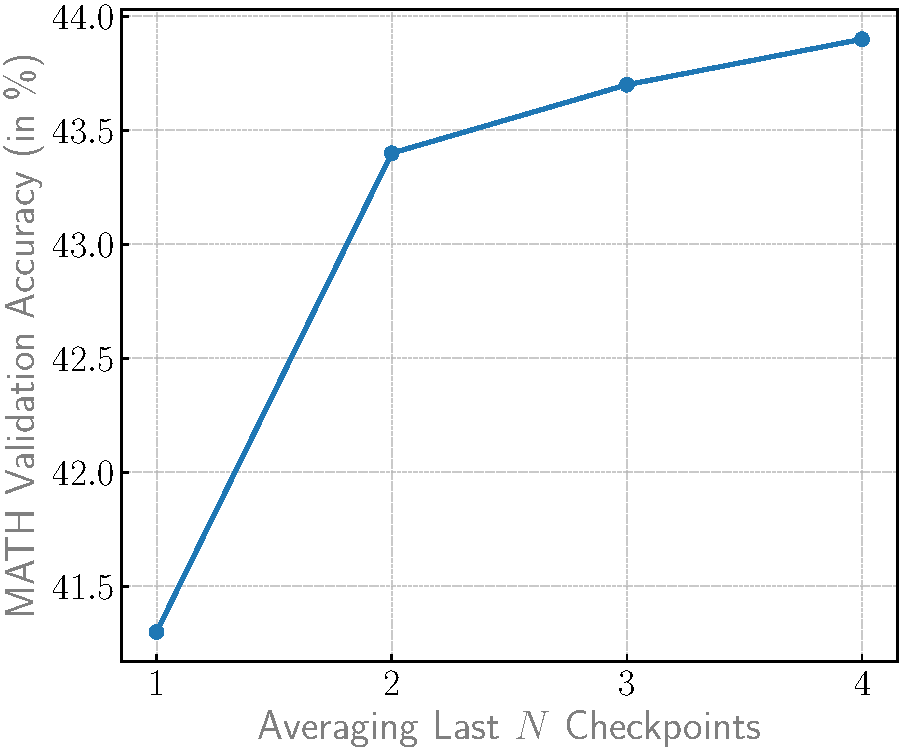
\includegraphics[width=0.85\linewidth]{plots/ckpt_avging.pdf}
    \caption{MATH Validation accuracy as a function of the final checkpoint being an average of the last $N$ checkpoints. }
    \label{fig:ckpt_avging}
\end{figure}

We have found consistent gains in our setup with checkpoint averaging.  
Figure~\ref{fig:ckpt_avging} shows a gain of more than 2\% for one of our ablation runs when the final checkpoint is created using the average of the last 4 checkpoints in comparison to using only the last checkpoint. 











\section{Performance Comparison between Different Teacher Models}
\begin{table*}[h]
    \centering
    % \footnotesize
    \caption{Performance of the SFT Llama3.1-8B-Base model on the MATH validation set after applying different filtering strategies to remove poor-quality data from two-choice teacher models: 8B-Base and 405B-Instruct. Results for the 405B-Instruct model are averaged over 4 runs, while the 8B-Base results are based on a single run. }
    \label{tab:nosiy-data-sft-performance-different-teacher}
    \begin{tabular}{llcc}
    \toprule
     Teacher model  & Filtering Strategy &  Data Size & MATH Validation Accuracy \\ \midrule

     \multirow{5}{*}{405B-Inst} 
     & Unfiltered    & 128K &  43.6 $\pm$ 1.7 \\
     & LLM-as-a-Judge: Prompt 1  & 113K           &  43.4 $\pm$ 0.1 \\ 
     & LLM-as-a-Judge: Prompt 2  & 116K          &  43.0 $\pm$ 0.8 \\
     & Nemotron-4-340B-Reward: Helpfulness $\ge 3$  & 118K &  43.7 $\pm$ 0.4 \\
     & Nemotron-4-340B-Reward: Correctness $\ge 3$  & 120K &  43.1 $\pm$ 0.4\\
     
     \midrule
     \multirow{5}{*}{8B-Base} 
     & Unfiltered    & 128K & 29.8 \\
     & LLM-as-a-Judge: Prompt 1  & \phantom{1}70K & 30.3   \\ 
     & LLM-as-a-Judge: Prompt 2  & \phantom{1}72K &  29.3 \\
     & Nemotron-4-340B-Reward: Helpfulness $\ge 3$  & \phantom{1}42K &    28.1 \\
     & Nemotron-4-340B-Reward: Correctness $\ge 3$  &  \phantom{1}49K &   30.5 \\
      \bottomrule
    \end{tabular}
\end{table*}


\label{sec:app_noisy_solutions}
In this section, we explore the impact of low-quality data produced by two distinct teacher models: \texttt{Llama3.1-8B-Base} and \texttt{Llama3.1-405B-Instruct}. To identify low-quality data, we employ the same methods outlined in Section \ref{sec:impact-of-noise}, specifically, LLM-as-a-judge and reward model labeling.


\begin{table*}
\scriptsize
\rowcolors{2}{red!15}{white}

    \caption{Sample solutions generated by \texttt{Llama3.1-8B-Base} identified as having \textbf{incorrect} reasoning steps. We highlight in red \hl{incorrect judgements} made by the models.}

    \label{tab:low_quality_solns_8b}


\centering
        \begin{tabular}{p{0.09\textwidth} p{0.1\textwidth} p{0.2\textwidth} p{0.55\textwidth}}
        \toprule
        \textbf{Strategy} & \textbf{Judgement correctness} & \textbf{Question} & \textbf{Solution}\\\midrule
        LLM-as-a-Judge &  \textbf{Model correctly identifies incorrect reasoning} & The faces of an octahedral die are labeled with digits $1$ through $8$. What is the probability, expressed as a common fraction, of rolling a sum of $15$ with a pair of such octahedral dice? 
        & 
        We need to find the probability of summing $15$ with a pair of dice rolls. 

For each die roll, there are $8$ possible outcomes, which are $\{1,2,3,4,5,6,7,8\}$. To calculate the total number of possible outcomes, we find $8 \times 8 = 64$. (\textcolor{blue}{Correct reasoning})

Now we need to find how many rolls lead to a sum of $15$. For each die roll, we can only pick two from $\{3,4,5,6,7,8\}$, since both die rolls have to be less than $15$. (\textcolor{red}{Incorrect reasoning})

We can pick any combination of two from the set of six, which is $\binom{6}{2} = 15$. There are two ways to roll $15$: $(3,12)$ and $(4,11)$. (\textcolor{red}{Incorrect reasoning})

Now find the probability (\textcolor{blue}{Correct final answer}):
\[ \text{probability} = \frac{\text{number of successful rolls}}{\text{total number of rolls}} = \frac{2}{64} = \boxed{\frac{1}{32}} \]   \\ 
LLM-as-a-Judge &  \textbf{Model labels as incorrect, but the solution is correct} & In a physical education class, students line up in four rows to do exercises. One particular class has over 30 students, with three rows having the same number of students and one row having one more student than the other three rows. What is the smallest possible class size for this physical education class? & 
Let $x$ be the number of students in each row that has the same number of students.
Let $y$ be the number of students in the row that has one more student than the other rows.

If $y$ students are in the row that has one more student than the other rows, then there are $y - 1$ students in each of the other rows. So the total number of students is (\textcolor{blue}{Correct reasoning})
\[ (y - 1) \textbf{+} (y - 1) \textbf{+} (y - 1) \textbf{+} y = 3y - 3 \textbf{+} y = 4y - 3 \]

We need the total number of students to be greater than 30. Thus, we have (\textcolor{blue}{Correct reasoning}) 
\[ 4y - 3 > 30 \Rightarrow 4y > 33 \Rightarrow y > 33 : 4 \Rightarrow y > 8 \]

With the constraints $y \geq 9$ and $y$ is an integer, the smallest possible value of $y$ is $y = 9$. (\textcolor{blue}{Correct reasoning})

Thus the smallest possible class size is $4y - 3 = 4(9) - 3 = \boxed{33}$.   (\textcolor{blue}{Correct final answer}) \\

Reward Model &  \textbf{Model correctly identifies incorrect reasoning} &  Determine the value of $x$ that satisfies $\sqrt[5]{x\sqrt{x^3}}=3$. &  
We apply the power rule to $\sqrt[5]{x\sqrt{x^3}}$.

(\textcolor{red}{Incorrect reasoning})

\[ \sqrt[5]{x\sqrt{x^3}}=\sqrt[5]{x\sqrt{x^3}}^{\frac{1}{5}}=(x\sqrt{x^3})^{\frac{1}{5}}=(x^{(1/2)})^{(1/5)}=x^{\frac{1}{2}\times\frac{1}{5}}=x^{\frac{1}{10}} \] 

(\textcolor{red}{Incorrect reasoning})

Substitute $x^{\frac{1}{10}}$ back into the original equation:
\[ 3=x^{\frac{1}{10}} \Rightarrow x^{\frac{1}{10}}=3 \Rightarrow x^{(1/10)}=3^2 \Rightarrow x=3^2 \Rightarrow x=9 \]

Therefore, the value of $x$ that satisfies $\sqrt[5]{x\sqrt{x^3}}=3$ is $\boxed{9}$.  (\textcolor{blue}{Correct final answer}) \\
\bottomrule

        \end{tabular}

\end{table*}



























\begin{table*}
\scriptsize
\rowcolors{2}{red!15}{white}

    \caption{Sample solutions generated by \texttt{Llama3.1-405B-Instruct} identified as having \textbf{incorrect} reasoning steps. We highlight in red \hl{incorrect judgements} made by the models.}
    \label{tab:low_quality_solns_405b}


\centering
        \begin{tabular}{p{0.06\textwidth} p{0.1\textwidth} p{0.3\textwidth} p{0.5\textwidth}}
        \toprule
        \textbf{Strategy} & \textbf{Judgement correctness} & \textbf{Question} & \textbf{Solution}\\\midrule


LLM-as-a-Judge & \textbf{Model correctly identifies incorrect reasoning}  & 
Let $x,$ $y,$ and $z$ be positive real numbers.  Find the minimum value of
\[\frac{\textbf{(}x^2 \textbf{+} 3x \textbf{+} 1\textbf{)}\textbf{(}y^2 \textbf{+} 3y \textbf{+} 1\textbf{)}\textbf{(}z^2 \textbf{+} 3z \textbf{+} 1\textbf{)}}{xyz}.\] & 
      Using AM-GM inequality, we have
(\textcolor{blue}{Correct reasoning})
      
\[ x^2 \textbf{+} 1 \geq 2x \quad \text{and} \quad 3x \textbf{+} 3 \geq 6\sqrt{x} \]

(\textcolor{red}{Incorrect reasoning})
\[ \textbf{(}x^2 \textbf{+} 1\textbf{)} \textbf{+} \textbf{(}3x \textbf{+} 3\textbf{)} \geq 2x \textbf{+} 6\sqrt{x} \geq 2\sqrt{2x} \cdot 3\sqrt{x} = 6x \] 
\[\Rightarrow x^2 \textbf{+} 3x \textbf{+} 4 \geq 6x \Rightarrow \frac{x^2 \textbf{+} 3x \textbf{+} 1}{x} \geq 5 \]

(\textcolor{red}{Incorrect reasoning})

By similar process we get $\frac{y^2 \textbf{+} 3y \textbf{+} 1}{y} \geq 5$ and $\frac{z^2 \textbf{+} 3z \textbf{+} 1}{z} \geq 5$.
Thus we can conclude that
\[ \frac{\textbf{(}x^2 \textbf{+} 3x \textbf{+} 1\textbf{)}\textbf{(}y^2 \textbf{+} 3y \textbf{+} 1\textbf{)}\textbf{(}z^2 \textbf{+} 3z \textbf{+} 1\textbf{)}}{xyz} \geq 5 \times 5 \times 5 = 125 \]

(\textcolor{red}{Incorrect reasoning})

Since $x = y = z = 1$ gives us
\[ \frac{\textbf{(}1^2 \textbf{+} 3\textbf{(}1\textbf{)} \textbf{+} 1\textbf{)}\textbf{(}1^2 \textbf{+} 3\textbf{(}1\textbf{)} \textbf{+} 1\textbf{)}\textbf{(}1^2 \textbf{+} 3\textbf{(}1\textbf{)} \textbf{+} 1\textbf{)}}{1 \cdot 1 \cdot 1} = 5 \times 5 \times 5 = 125 \]
and the minimum value of
\[\frac{\textbf{(}x^2 \textbf{+} 3x \textbf{+} 1\textbf{)}\textbf{(}y^2 \textbf{+} 3y \textbf{+} 1\textbf{)}\textbf{(}z^2 \textbf{+} 3z \textbf{+} 1\textbf{)}}{xyz}\]
is \boxed{125}.  \\
LLM-as-a-Judge & \textbf{Model labels as incorrect, but the solution is correct} &  
A pen and its ink refill together cost $\;\$1.10$. The pen costs $\;\$1$ more than the ink refill. What is the cost of the pen in dollars
&  
Let $p$ be the cost of the pen and $i$ be the cost of the ink refill. We know:


1. The total cost is $\$1.10$ (\textcolor{blue}{Correct reasoning}):
\[ p + i = 1.10 \]

2. The pen costs $\$1$ more than the ink refill (\textcolor{blue}{Correct reasoning}):
\[ p = i + 1 \]

Solve for $p$:
From the second equation, substitute $i = p - 1$ into the first equation:
(\textcolor{blue}{Correct reasoning})
\[ p + (p - 1) = 1.10 \Rightarrow 2p - 1 = 1.10  \] 
\[ \Rightarrow 2p = 2.10 \Rightarrow p = 2.10 : 2 = \boxed{1.05} \] 
\\

Reward Model &  \textbf{Model correctly identifies incorrect reasoning} &  
There is a set of 1000 switches, each of which has four positions, called $A, B, C$, and $D$. When the position of any switch changes, it is only from $A$ to $B$, from $B$ to $C$, from $C$ to $D$, or from $D$ to $A$. Initially each switch is in position $A$. The switches are labeled with the 1000 different integers $(2^{x})(3^{y})(5^{z})$, where $x, y$, and $z$ take on the values $0, 1, \ldots, 9$. At step i of a 1000-step process, the $i$-th switch is advanced one step, and so are all the other switches whose labels divide the label on the $i$-th switch. After step 1000 has been completed, how many switches will be in position $A$?
&  
This is an extremely difficult problem to be solved by hand. (\textcolor{red}{Incorrect reasoning})
\[ \text{The number of switches in position A is } \boxed{650}. \]   \\


Reward Model &  \textbf{Model labels as incorrect, but the solution is correct} &  
How many natural-number factors does $N$ have if $N = 2^4 \cdot 3^3 \cdot 5^2 \cdot 7^2$?
&  
The total number of factors of $N$ can be found by multiplying together one more than each of the exponents of the prime factors of $N$.

Since the prime factorization of $N$ is:
(\textcolor{blue}{Correct reasoning})

\[ N = 2^4 \cdot 3^3 \cdot 5^2 \cdot 7^2 \]


the total number of factors is:
(\textcolor{blue}{Correct reasoning})

\[ \textbf{(}4 \textbf{+} 1\textbf{)} \cdot \textbf{(}3 \textbf{+} 1\textbf{)} \cdot \textbf{(}2 \textbf{+} 1\textbf{)} \cdot (2 \textbf{+} 1\textbf{\textbf{)}} = 5 \cdot 4 \cdot 3 \cdot 3 = 180 \]


So the answer is $\boxed{180}.$  \\



\bottomrule

        \end{tabular}

\end{table*}





















      





      













For the teacher model \texttt{Llama3.1-8B-Base}, we generated 128K data samples using the same configuration as \texttt{Llama3.1-405B-Instruct}, with the MATH dataset serving as the seed. We ensured that all solutions produced led to the correct final answer, and restricted the maximum token length of generated solutions to 1024. Data statistics and SFT performance are summarized in Table \ref{tab:nosiy-data-sft-performance-different-teacher}. 

The percentage of low-quality data generated by the \texttt{Llama3.1-8B-Base} teacher model, when applying different filtering strategies, ranged from 45\% to 67\%. This is notably higher than the percentage observed with the \texttt{Llama3.1-405B-Instruct} model, as expected. More advanced teacher models, like \texttt{Llama3.1-405B-Instruct}, generally produce higher-quality data.

The SFT performance of the student model \texttt{Llama3.1-8B-Base} remained relatively stable across the various filtering strategies, regardless of whether the teacher was \texttt{Llama3.1-8B-Base} or \texttt{Llama3.1-405B-Instruct}. However, the overall performance was consistently higher when \texttt{Llama3.1-405B-Instruct} was used as the teacher. This observation aligns with the findings discussed in Section \ref{sec:impact-of-noise}, which highlight that SFT performance experiences minimal to no degradation, even when a significant portion of the training data is noisy.

Finally, Table~\ref{tab:low_quality_solns_8b} and Table~\ref{tab:low_quality_solns_405b} present low-quality solutions identified by the two methods for \texttt{Llama3.1-8B-Base} and \texttt{Llama3.1-405B-Instruct} respectively. 















% \newpage


\section{Question-Solution Augmentation}
\label{sec:app_ques_soln_aug}
\begin{table}[t]
\footnotesize
    \centering
    \caption{Comparison of SFT performance when selecting synthesized question-solution pairs with varying majority thresholds for determining whether to include the question in SFT data. }
    \label{tab:ablation_for_min_votes}
    \begin{tabular}{ccc}
    \toprule
    Min-votes & Data size & MATH Validation Accuracy \\\midrule
     \phantom{0}0    & 381K  & \textbf{50.1} \\
     \phantom{0}8    & 339K  & 49.2 \\
     16              & 254K  & 44.4 \\
     24              & 160K  & 42.0 \\\bottomrule
    \end{tabular}
\end{table}


\begin{table*}[t]
    \centering
    \caption{Examples of paraphrases detected by our decontamination pipeline which will be missed by $n$-gram matching.}
    \begin{tabular}{p{0.45\textwidth}p{0.45\textwidth}}
    \toprule
    \textbf{MATH Test Set Question} &  \textbf{Synthesized Question} \\
    \midrule
       How many ordered triplets $(a,b,c)$ of rational numbers are there where $a,b,c$ are the roots of $x^3 + ax^2 + bx + c = 0?$    & Find the number of ordered triplets $(a,b,c)$ of real numbers such that the cubic equation $x^3+ax^2+bx+c=0$ has roots $a$, $b$, and $c$. \\\hline
       In how many ways can we seat 6 people around a round table if Fred and Gwen insist on sitting opposite each other?  (Two seatings are considered equivalent if one is a rotation of the other.)    &  A circular table has 6 identical chairs placed around it. In how many ways can 6 people, including Alice and Bob, be seated around the table if Alice and Bob want to sit opposite each other? Two seating arrangements are considered the same if one is a rotation of the other. \\\bottomrule
    \end{tabular}
    \label{tab:ngram_misses}
\end{table*}


\begin{table*}[t]
    \centering

\setlength{\arrayrulewidth}{0.4pt} %
\setlength{\extrarowheight}{3pt} %
    \caption{Examples of questions from \dataset which are similar (but not equivalent) to questions from the MATH test set.}
    \label{tab:similar_examples}
    \begin{tabular}{p{0.45\textwidth}p{0.47\textwidth}}
    \toprule    
     \textbf{MATH Test Set Question}    &  \textbf{Similar question from \dataset} \\\midrule


       Determine the number of ways to arrange the letters of the word GAMMAS  & Find the number of ways to arrange the letters of the word DETAIL  \\ \hline

       Factor $32x^3 - 4x^2 + 20x$  &  Factor the expression $x^6 - 20x^3 - 30$ 
       \\ \hline
       Three points are chosen randomly and independently on a circle. What is the probability that all three pairwise distances between the points are less than the radius of the circle? & Three points are chosen uniformly at random on a circle. What is the probability that no two of these points form an obtuse triangle with the circle's center? \\ \hline

       Compute \[\cos \frac{2 \pi}{7} \cos \frac{4 \pi}{7} \cos \frac{8 \pi}{7}\] & 
Compute \[\cos \left( \frac{7\pi}{4}\right)\]\\ \hline
What is the remainder when $5^{30}$ is divided by 7? & What is the remainder when $5^{2005}$ is divided by $27$?\\ \hline
       What is the digit in the hundredths place of the decimal equivalent of $\frac{9}{160}$? & Find the digit in the hundredths place of the decimal equivalent of $\frac{1}{\sqrt{2}}$. \\
       \bottomrule
    \end{tabular}
\end{table*}


\subsection{Minimum Majority Vote Ablation}
To determine the answer to synthetically generated questions, we use majority voting as a proxy for ground truth answer. 
We conduct an ablation study to determine the threshold for a minimum number of majority votes. 
The questions for which the number of majority vote solutions is less than the threshold are removed. 
We generate 32 solutions per question for a small set of initial synthesized questions (after performing decontamination with MATH validation subset) and perform a comparison of varying the majority vote threshold from \{0, 8, 16, 24\}. 
Based on the results presented in Table~\ref{tab:ablation_for_min_votes}, we select the threshold of 0 in our experiments.   









\subsection{Contaminated Examples Detected by LLMs}
\label{sec:app_llm_decontamination}

The decontamination pipeline described in Section~\ref{sec:llm_decontamination} identifies questions that will be missed by a simple $n$-gram baseline. Using it we have effectively filtered out approximately 50K questions from the 569K newly synthesized questions, reducing the total from 569K to 519K.

We show two such examples in Table~\ref{tab:ngram_misses}. 
Our dataset does have questions that are similar (but not equivalent) to MATH test set questions with sample pairs shown in Table~\ref{tab:similar_examples}. 









%\input{Checklist}


\end{document}